\PassOptionsToPackage{unicode=true}{hyperref} % options for packages loaded elsewhere
\PassOptionsToPackage{hyphens}{url}
%
\documentclass[]{article}
\usepackage{lmodern}
\usepackage{amssymb,amsmath}
\usepackage{ifxetex,ifluatex}
\usepackage{fixltx2e} % provides \textsubscript
\ifnum 0\ifxetex 1\fi\ifluatex 1\fi=0 % if pdftex
  \usepackage[T1]{fontenc}
  \usepackage[utf8]{inputenc}
  \usepackage{textcomp} % provides euro and other symbols
\else % if luatex or xelatex
  \usepackage{unicode-math}
  \defaultfontfeatures{Ligatures=TeX,Scale=MatchLowercase}
\fi
% use upquote if available, for straight quotes in verbatim environments
\IfFileExists{upquote.sty}{\usepackage{upquote}}{}
% use microtype if available
\IfFileExists{microtype.sty}{%
\usepackage[]{microtype}
\UseMicrotypeSet[protrusion]{basicmath} % disable protrusion for tt fonts
}{}
\IfFileExists{parskip.sty}{%
\usepackage{parskip}
}{% else
\setlength{\parindent}{0pt}
\setlength{\parskip}{6pt plus 2pt minus 1pt}
}
\usepackage{hyperref}
\hypersetup{
            pdftitle={Incentivos al Retiro},
            pdfborder={0 0 0},
            breaklinks=true}
\urlstyle{same}  % don't use monospace font for urls
\usepackage[margin=1in]{geometry}
\usepackage{graphicx,grffile}
\makeatletter
\def\maxwidth{\ifdim\Gin@nat@width>\linewidth\linewidth\else\Gin@nat@width\fi}
\def\maxheight{\ifdim\Gin@nat@height>\textheight\textheight\else\Gin@nat@height\fi}
\makeatother
% Scale images if necessary, so that they will not overflow the page
% margins by default, and it is still possible to overwrite the defaults
% using explicit options in \includegraphics[width, height, ...]{}
\setkeys{Gin}{width=\maxwidth,height=\maxheight,keepaspectratio}
\setlength{\emergencystretch}{3em}  % prevent overfull lines
\providecommand{\tightlist}{%
  \setlength{\itemsep}{0pt}\setlength{\parskip}{0pt}}
\setcounter{secnumdepth}{0}
% Redefines (sub)paragraphs to behave more like sections
\ifx\paragraph\undefined\else
\let\oldparagraph\paragraph
\renewcommand{\paragraph}[1]{\oldparagraph{#1}\mbox{}}
\fi
\ifx\subparagraph\undefined\else
\let\oldsubparagraph\subparagraph
\renewcommand{\subparagraph}[1]{\oldsubparagraph{#1}\mbox{}}
\fi

% set default figure placement to htbp
\makeatletter
\def\fps@figure{htbp}
\makeatother


\title{Incentivos al Retiro}
\author{}
\date{\vspace{-2.5em}}

\begin{document}
\maketitle

{
\setcounter{tocdepth}{3}
\tableofcontents
}
\hypertarget{introducciuxf3n}{%
\section{Introducción}\label{introducciuxf3n}}

Importancia de alargar vida laboral, OECD (2011).

Desde la década de 1980 se acumula evidencia de que los Sistemas
Jubilatorios y los incentivos que generan para los trabajadores son un
factor determinante de la oferta laboral de los mayores de 55 años.

Muchos países implementaron cambios en el diseño y los parámetros de sus
sistemas jubilatorios para incentivar a los mayores continuar en el
mercado laboral.

Presentamos la evidencia de los resultados de estas políticas.

\hypertarget{tendencias}{%
\section{Tendencias}\label{tendencias}}

Envejecimiento poblacional.

\hypertarget{esperanza-de-vida-de-los-mayores-y-tiempo-esperado-de-retiro}{%
\subsection{Esperanza de vida de los mayores y tiempo esperado de
retiro}\label{esperanza-de-vida-de-los-mayores-y-tiempo-esperado-de-retiro}}

Si bien en la primera parte del siglo pasado los aumentos en la
esperanza de vida fueron causados principalemnte por caídas en la
mortalidad infantil, a partir de mitad de siglo, también hubo caídas
importantes en la mortalidad de los mayores (OECD (2011)).

En efecto, en los países de la OCDE, la esperanza de vida a los 65 años
de edad aumentó 3.9 años para los hombres y 5.4 para las mujeres entre
1960 y 2010 (OECD (2011)). En Uruguay, COMPLETAR.

\hypertarget{la-actividad-laboral-de-los-mayores}{%
\subsection{La actividad laboral de los
mayores}\label{la-actividad-laboral-de-los-mayores}}

Otro factor que impacta directamente en la sostenibilidad financiera de
los sistemas jubilatorios, es la participación laboral de los mayores,
sensiblemente menores a las de los más jóvenes.

La participación de los mayores en el mercado laboral ha seguido un
patrón de U desde los años 70s del siglo XX. La caída pronunciada hasta
los años 90s se revirtió en mucho países, conformando un patrón en forma
de U (Börsch-Supan and Coile (2019)). En los apartados X y Y,
presentamos la evidencia disponible sobre el impacto de los incentivos
producidos por los sistemas previsionales en este fenómeno.

El siguiente gráfico muestra el aumento de la tasa de actividad en las
personas de entre 55 y 64 años en varios países.

Sin embargo, estos aumentos no compensan el aumento en la longevidad
mencionados anteriormente. Aún con edades de retiro efectivas mayores,
OCDE proyecta que la esperanza de vida luego de la edad normal de retiro
aumente en la mayoría de los países miembro (OECD (2019)).

Sin embargo, en 2011 sólo 5 países de la OCDE -Hungría, Italia, Corea
del Sur, Turquía y el Reino Unido- habían logrado aumentar estas edades
suficiente para estabilizar la duración esperada de los períodos de
retiro. El aumento del tiempo esperado de retiro amenaza la
sostenibilidad fiscal de los sistemas previsionales de reparto.

\hypertarget{poluxedticas-para-favorecer-el-empleo-de-los-mayores}{%
\subsection{Políticas para favorecer el empleo de los
mayores}\label{poluxedticas-para-favorecer-el-empleo-de-los-mayores}}

En la década de 1970 y 1980 muchos países desarrollados flexibilizaron
el acceso a las jubilaciones para favorecer el empleo juvenil. (CITA).
Esta flexibilización se hizo mediante la rebaja de las edades mínimas de
eligibilidad, el acceso a otros programas de seguridad social y la
eliminación de ajustes actuariales por el retiro temprano.

Si bien los efectos esperados sobre el empleo juvenil no se
materializaron, si se produjo una caída importante de la edad de retiro
del mercado laboral. El gráfico siguiente muestra la edad de retiro
proyectadas de los países de la OCDE entre 1950 a 2050. El mínimo se
alcanzó en 1993, y no se espera que se recuperen las edades de 1950
hasta 2050.

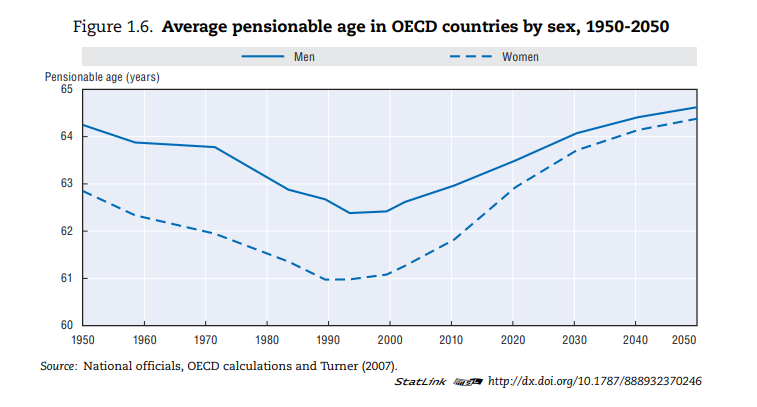
\includegraphics{imgs/pensions-glance-fig1.6.png}

En la década de 1990 empezó a surgir evidencia de que las reglas de los
sistemas jubilatorios generaban incentivos al retiro temprano y eran uno
de los principales factores que explicaban la caída en la participación
laboral de los mayores (({\textbf{???}})).

Esta caída, combinada con el aumento en la longevidad mencionado antes
impactaba directamente en la sostenibilidad de los sistemas jubilatorios
de reparto.

Para aliviar este problem, a partir de los años 2000 se empiezan a
implementar medidas para revertir este fenómeno, favoreciendo el
alargamiento de la vida laboral de las personas. En particular, las
edades a los que los trabajadores pueden acceder a distintos niveles de
beneficios en los sistemas jubilatorios son un parámetro clave para la
decisión de los trabajadores de retirarse del mercado laboral y/o
acogerse a estos beneficios.

\hypertarget{edad-muxednima-de-retiro}{%
\subsubsection{Edad Mínima de Retiro}\label{edad-muxednima-de-retiro}}

En este contexto, La edad mínima de retiro surge como un parámetro clave
en cualquier sistema previsional. Es la menor edad a la que un
trabajador puede recibir una prestación del sistema jubilatorio. Si bien
este suele ser un parámetro muy saliente en todo sistema previsional, es
usual que los trabajadores cuenten con otros vías para retirarse del
mercado laboral antes de esta edad (seguro de desempleo prolongado, ,
seguro de enfermedad, pensiones por invalidez, etc.). En muchos países,
estas vías terminan funcionando como esquemas de retiro temprano.

El siguiente gráfico muestra la EMR de los países de la OCDE en 2018. El
promedio es XX. La tendencia en las últimas décadas fue aumentar esta
edad (OECD (2019)).

\hypertarget{edad-normal-de-retiro-e-incentivos-a-diferir-el-retiro}{%
\subsubsection{Edad Normal de Retiro e incentivos a diferir el
retiro}\label{edad-normal-de-retiro-e-incentivos-a-diferir-el-retiro}}

La Edad Normal de Retiro es la menor edad a la que un trabajador puede
acceder a una prestación del sistema jubilatorio sin recibir
penalizaciones por retiro temprano. Uno de los hechos estilizados
encontrado en la literatura es que una gran proporción de los
trabajadores se retira la EMR o la ENR.

Para Uruguay, ver ({\textbf{???}}). En este contexto, aumentar estas
edades surge como una medida con potencial de ser altamente eficaz para
prolongar la vida laboral de los trabajadores.

La estructura de ests ajustes definen los incentivos a diferir el
retiro, ya que penalizan el retiro temprano y estimulan el retiro
tardío.

{[}Pensions at a glance 2019 fig 1.12{]}

El siguiente gráfico muestra el aumento en la tasa efectiva y normal de
retiro promedio en los países de la OCDE. ({\textbf{???}})

{[}Pensions at a glance fig 2.6.{]}

\hypertarget{impacto-de-la-seguridad-social-en-la-oferta-de-trabajo}{%
\section{Impacto de la Seguridad Social en la oferta de
trabajo}\label{impacto-de-la-seguridad-social-en-la-oferta-de-trabajo}}

\hypertarget{marco-teuxf3rico}{%
\subsection{Marco Teórico}\label{marco-teuxf3rico}}

El marco teórico mas usado para analizar el impacto de los parámetros de
los sistemas previsionales en las decisiones de retiro es un modelo en
el que el trabajador representativo maximiza la utilidad derivada del
consumo de bienes y de ocio.

La utilidad del trabajador depende positivamente de ambos. Si decide
trabajar más, puede consumir más pero se ve obligado a disfrutar de
menos ocio, por lo que existe un \emph{trade off} entre ambos bienes.

El sistema jubilatorio afecta esta decisión a través de dos canales: el
precio relativo de ambos bienes y la riqueza total del individuo. En
efecto, si el sistema penaliza más el trabajo, el ocio se vuelve más
barato relativo al consumo. Por otro lado, si las prestaciones del
sistema se reducen, el precio relativo de ambos bienes se mantiene pero
el trabajador va a acceder a un menor nivel de ambos.

Este modelo se puede extender para analizar fenómenos más complejos. En
primer lugar, el modelo supone que no hay restricciones de liquidez.
Esto implica que el trabajador tiene acceso al mercado financiero, lo
que le permite suavizar su consumo. Si, por el contrario, el trabajador
enfrenta restricciones de liquidez, es posible que se vea obligado a
seguir en el mercado de trabajo por más tiempo para mantener sus niveles
de consumo.

Por otro lado, el modelo no permite analizar decisiones conjuntas de
miembros de un mismo hogar. Algunos trabajos extienden este modelo para
analizar los impactos de los sistemas de seguridad social en los
hogares. En este marco, si el ocio de uno de los integrantes del hogar
es un bien complementario al del otro, los incentivos que enfrenta uno
de los integrantes del hogar afectan a otros. Esto permite explicar
como, por ejemplo, algunas parejas deciden retirarse juntas.

Otro fenómeno relevante es el de señalización. En este marco, las edades
de retiro dispuestas en las reglas de los sistemas jubilatorios actúan
como señales para que los trabajadores se retiren.

Finalmente, otro de los aspectos importantes a tener en cuenta en la
decisión de retiro es la existencia de oportunidades en el mercado de
trabajo para los trabajadores. Estos aspectos implican tomar en cuenta
la demanda de trabajo de parte de las empresas y la discriminación que
pueden sufrir los trabajadores mayores en el mercado de trabajo.

\hypertarget{midiendo-los-incentivos-de-la-seguridad-social}{%
\subsection{Midiendo los incentivos de la Seguridad
Social}\label{midiendo-los-incentivos-de-la-seguridad-social}}

Importancia de elegir los incentivos correctamente desde el punto de
vista de la equidad y la eficiencia. La eficiencia implica que los
ingresos obtenidos del sistema jubilatorio guarde relación con los
aportes realizados durante la vida activa, y que no haya incentivos al
retiro temprano.

La equidad implica asegurar un nivel de consumo adecuado a todos los
mayores.

\hypertarget{tasa-de-reemplazo}{%
\subsubsection{Tasa de Reemplazo}\label{tasa-de-reemplazo}}

El indicador más simple para medir los incentivos que enfrentan los
trabajadores a la hora de retirarse es la tasa de reemplazo. Esta tasa
mide la relación entre lo que percibe en el mercado laboral y lo que
recibe como prestación una vez que se acoge a los beneficios del sistema
previsional.

En la mayor parte esta tasa es creciente con la edad. En Uruguay,
COMPLETAR. Sin embargo, este no es el único parámetro que los
trabajadores tienen en cuenta cuando deciden retirarse.

\hypertarget{riqueza-jubilatoria-y-el-impuesto-impluxedcito-al-trabajo}{%
\subsubsection{Riqueza Jubilatoria y el impuesto implícito al
trabajo}\label{riqueza-jubilatoria-y-el-impuesto-impluxedcito-al-trabajo}}

Para entender mejor esta decisión, es necesario tomar en cuenta el
concepto de Riqueza de la Seguridad Social o Riqueza Jubilatoria. Esto
es el valor presente de todos los pagos que recibe un trabajador del
sistema de jubilatorio. La Riqueza de la Seguridad Social (SSW) para una
edad de retiro \(h\) es el valor actualizado de los beneficios recibidos
entre \(h + 1\) y la fecha de muerte \(S\), si el trabajador se retira a
la edad \(h\):

\[ SSW_{h} = \sum_{s=h+1}^{\S} \rho_{s} B_{s}(h)\]

Para actualizar los beneficios se utiliza el factor de descuento
\(\rho\), que depende de la probabilidad de sobrevivencia y el factor de
descuento intertemporal.

Una medida de incentivos fundamental es el cambio de la Riqueza
Jubilatoria que obtiene un trabajador por diferir su retiro. El
devengamiento de \(SSW\) es la medida más simple de incentivo a
trabajar, consiste en calcular el cambio en SSW por permanecer en la
fuerza de trabajo un año más:

\[ SSA_{a} = SSW_{a+1} - SSW_{a}\]

\begin{itemize}
\tightlist
\item
  Gruber and Wise (2004) and Samwick (1998) argue that the accrual
  effect is the main driving source of retirement behavior in the
  reforms.
\end{itemize}

Este cambio depende de las características del trabajador y su
interacción con las reglas del sistema que lo cubre y puede resultar del
prolongamiento del tiempo de actividad o de la reducción del tiempo
durante el que se reciben beneficios.

El impacto más importante de esta decisión es la caída en la Riqueza
Jubilatoria por el período por el que el trabajador difiera el retiro.

En un sistema de capitalización individual, por ejemplo, trabajar un año
más implica que la cuenta de ahorro del trabajador recibe un año más de
aportes, y estos aportes se capitalizan un año más por el rendimiento
que obtienen estos ahorros. Por otro lado, la anualidad que recibirá el
trabajador estará calculada en base a una esperanza de vida un año
mayor, por lo que será más alta.

En sistemas de reparto, los incentivos que enfrenta el trabajador para
trabajar un año más son diferentes. Estos incentivos dependen de la
forma en que se actualizan los aportes realizados durante la vida del
trabajador para calcular el sueldo jubilatorio, la forma en que se tomen
en cuenta la historia laboral del individuo para este cálculo, y, en
sistemas nocionales, el rendimiento de los aportes en el período en el
que el trabajador difiere su retiro.

El impuesto implícito a seguir trabajando se calcula como:

\[ \tau_{a} = \frac{-SSA_{a}}{W_{a+1}} \]

Acá va la figure de micro estimation.

En algunos países, los sistemas jubilatorios implican pruebas de
ingresos o de activos, o, como en Uruguay, existen trabas legales a que
los trabajadores perciban ingresos del sistema jubilatorio mientras se
mantienen activos.

En otros países, la decisión de retirarse del mercado de trabajo es
independiente de la decisión de acogerse a los beneficios del sistema
jubilatorio (UK, Noruega), por lo que la definición de retiro no implica
una sino dos decisiones.

\hypertarget{medidas-muxe1s-sofisticadas-peak-value-y-option-value}{%
\subsubsection{Medidas más sofisticadas: Peak Value y Option
Value}\label{medidas-muxe1s-sofisticadas-peak-value-y-option-value}}

El principal problema que tiene es que esta medida solo mira un período
para adelante, pero la SSA no se incrementa monotónicamente, sino que
puede tener saltos.

Eso implica que para un trabajador la SSA de un año puede ser baja, pero
la de 4 años para adelante tener un salto brusco, por lo que el
trabajador sigue trabajando teniendo ese salto en cuenta.

Es la diferencia máxima entre la riqueza de la seguridad social de
retirarse hoy o retirarse en otra fecha:

\[ PV_{a} = max_{h}(SSW_{h}-SSW_{a}) \]

Propuesta por Stock and Wise (1990): Option Value.

Resultados empíricos usando estas medidas (Gruber and Wise (2004)).

\begin{itemize}
\tightlist
\item
  Para América Latina: Cerda, Muñoz, etc.
\end{itemize}

\begin{itemize}
\tightlist
\item
  Salida de Microestimation
\end{itemize}

\hypertarget{evidencia-reciente}{%
\subsection{Evidencia Reciente}\label{evidencia-reciente}}

Problemas de la evidencia anterior. Ex-ante, basada en simulaciones. La
evidencia más reciente consiste en evaluar los efectos observados de
medidas efectivamente implementadas.

Los estudio ex-ante estiman menores impactos de la seguridad social en
la participación laboral. Principales razones que atenúan las
estimaciones:

Primero, no capturan efectos de posibles señales o normas sociales que
generan las edades mínimas y normales. Segundo, los cálcuos de las
medidas de incentivos tienen error de medida por falta de información
sobre los contribuyentes (estructura familiar, etc.).

Tercero y más importante las estimaciones tienen sesgos de endogeneidad
por las correlaciones entre las historias laborales, las preferencias
por el trabajo y los incentivos al retiro.

En las últimas décadas, muchos países implementaron reformas
paramétricas para estimular la participación laboral de los mayores.
Estas reformas generaron una literatura creciente en los últimos años
que usa diseños cuasi-experimentales para evaluar el impacto de estos
cambios paramétricos en la participación laboral de los individuos.

\hypertarget{impacto-de-edad-muxednima-de-retiro}{%
\subsubsection{Impacto de Edad Mínima de
Retiro}\label{impacto-de-edad-muxednima-de-retiro}}

Rabaté, Staubli, \ldots{}

\hypertarget{impacto-de-incentivos-financieros-y-cambios-en-la-edad-normal-de-retiro}{%
\subsubsection{Impacto de incentivos financieros y cambios en la Edad
Normal de
Retiro}\label{impacto-de-incentivos-financieros-y-cambios-en-la-edad-normal-de-retiro}}

Resumen de Mastrobuoni (2009), Hanel (2010).

\hypertarget{lecciones-para-uruguay}{%
\section{Lecciones para Uruguay}\label{lecciones-para-uruguay}}

\begin{itemize}
\tightlist
\item
  La edad mínima de jubilación es un instrumento altamente eficaz para
  prolongar la vida laboral de los mayores. Efecto señalización es parte
  del impacto.
\item
  Los incentivos actuariales también funcionan.
\item
  Jubilaciones mínimas pueden ser un incentivo a salir temprano del
  mercado a pesar de los ajustes actuariales.
\item
  Ojo con los otros programas.
\item
  Salud y educación, restricciones en las oportunidades de empleo.
\end{itemize}

\hypertarget{glosario}{%
\section{Glosario}\label{glosario}}

\begin{description}
\item[Edad Efectiva de Retiro]
Es la edad a la que un individuo empieza a recibir prestaciones del
sistema de seguridad social.
\item[Edad Mínima de Retiro]
Es la menor edad a la que un trabajador puede aplicar a un programa de
seguridad social. Es usual que en estos casos las prestaciones se vean
reducidas frente a las recibidas en la edad normal de retiro.
\item[Retiro Temprano]
Es la práctica de acogerse a los beneficios de la seguirdad social antes
de la edad normal de retiro.
\item[Prueba de Ingresos]
Es un límite a los ingresos que puede tener alguien que recibe
prestaciones del sistema de segurida social.
\item[Impuestos Implícitos]
Es el impuesto implícito que enfrenta un trabajador cuando, pudiendo
recibir una prestación del sistema de seguirdad social, decide seguir
trabajando y sus beneficios futuros no son compensados.
\item[Riqueza Jubilatoria]
Es el valor descontado al momento del retiro de las prestaciones que
recibe el contribuyente del sistema jubilatorio.
\end{description}

\hypertarget{referencias}{%
\section*{Referencias}\label{referencias}}
\addcontentsline{toc}{section}{Referencias}

\hypertarget{refs}{}
\leavevmode\hypertarget{ref-NBERc14190}{}%
Börsch-Supan, Axel, and Courtney Coile. 2019. ``Introduction to 'Social
Security Programs and Retirement Around the World: Reforms and
Retirement Incentives'.'' In \emph{Social Security Programs and
Retirement Around the World: Reforms and Retirement Incentives}.
University of Chicago Press. \url{http://www.nber.org/chapters/c14190}.

\leavevmode\hypertarget{ref-gruber04}{}%
Gruber, Jonathan, and David Wise. 2004. ``Social Security Programs and
Retirement Around the World: Micro Estimation.''

\leavevmode\hypertarget{ref-hanel09}{}%
Hanel, Barbara. 2010. ``Financial Incentives to Postpone Retirement and
Further Effects on Employment---Evidence from a Natural Experiment.''
\emph{Labour Economics} 17: 474--86.

\leavevmode\hypertarget{ref-mastrobouni09}{}%
Mastrobuoni, Giovanni. 2009. ``Labor Supply Effects of the Recent Social
Security Benefit Cuts: Empirical Estimates Using Cohort
Discontinuities.'' \emph{J. Public Econ.} 93 (11-12): 1224--33.

\leavevmode\hypertarget{ref-ocde11}{}%
OECD. 2011. ``Pensions at a Glance 2011.''

\leavevmode\hypertarget{ref-ocde19}{}%
---------. 2019. ``Pensions at a Glance 2019.''

\leavevmode\hypertarget{ref-stock90}{}%
Stock, J.H., and D.A. Wise. 1990. ``Pensions, the Option Value of Work,
and Retirement.'' \emph{Econometrica} 58 (5): 1151--1180.

\end{document}
